%
% clip.tex
%
% (c) 2024 Lukas Schöpf, OST Ostschweizer Fachhochschule
%


\chapter{Cross-modal networks
    \label{chapter:crossmodalnetworks}}
    Multimodal deep learning is the study of models that learn from multiple modalities.
    For example, a human can use both vision and hearing to identify an object or a person.
    Cross-modal deep learning, on the other hand, uses data from one modality to improve performance in another.
    For example, if a human looks at a picture of a bird and listens to the bird's song, they might be able to identify the bird.

    Its most impressive feature is the ability to perform well on data on which the model has not been trained.
    This ability is called zero-shot capability, which is derived from N-shot capability.
    N-shot capability describes how many training samples of a particular class a model needs to classify it correctly.

    In this work, cross-modal networks are used to find relationships between images and text.
    Most cross-modal networks built for this task consist of a text encoder and an image encoder.

    \section{Text encoder}
    The text encoder is in most cases a transformer (see \cref{fig:crossmodalnetworks:textencoder}).
    It encodes a given text into a high dimensional vector space.
    The closer 2 words are related, the closer their embedded vectors are to each other.
    This high dimensional vector space allows the transformer to classify unseen classes quit correctly because their vector is close to related classes.
    For example the vector for cat shoud be close to the vector for dog.

    \begin{figure}
        \centering
        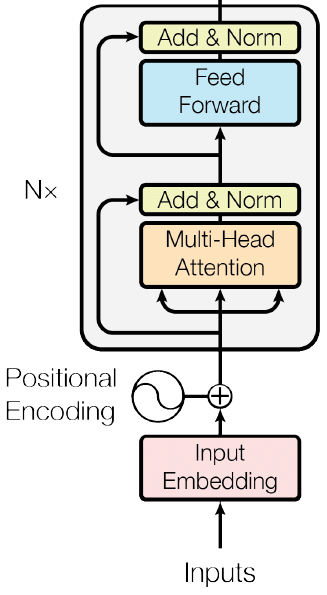
\includegraphics[width=0.25\textwidth]{Images/crossmodalnetworks/The-Transformer-encoder-structure.png}
        \caption{Image of a transformer used as a textencoder\cite{fig:encoder}.}
        \label{fig:crossmodalnetworks:textencoder}
    \end{figure}
    


    \section{Image encoder}
    The image encoder consists of a vision transformer\cite{Vis_N_Grams} in most cases.
    As the text encoder the vision encoder encodes a image in a high dimensional vector space.



    \section{CLIP
        \label{section:clip}}
    \acrfull{clip} \cite{clip} is a cross-modal model from openAI\cite{openai} which can tell how well a given image and a given text fit together.
    Its can be used with a variaty of image and text encoders.
    It is trained on a large Dataset, which consist of 400 million image-text pairs.
    On its realeas it outperformed some of the best models known 
    Many other model use CLIP as their base and build better models of it.




    \section{ALIGN
        \label{section:align}}

    \begin{table}
        \begin{tabular}{llll}
            \hline
        &  a Yahoo& ImageNet& SUN \\\hline
        Visual N-Grams&  72,4&  11,5&  23,0\\
        CLIP&  98,4&  76,2&58,5\\ \hline
        \end{tabular}
        \caption{Table 1. from \cite{clip}. Comparing CLIP to prior image zero-shot classification results\cite{Vis_N_Grams}}
    \end{table}